\documentclass{ximera}
\title{Algebra of Functions and Composition}

\outcome{Add, subtract, multiply, and divide functions and determine the domain of the result.}
\outcome{Evaluate composed functions from formulas, graphs, and tables.}
\outcome{Find the domain of a composed function.}
\outcome{Decompose a function into a composition of simpler functions.}
\outcome{Compute and simplify the difference quotient.}

\begin{document}
\begin{abstract}
\end{abstract}
\maketitle

\textbf{Learning Objectives:}
\begin{itemize}
  \item Add, subtract, multiply, and divide functions and determine the domain of the result.
  \item Evaluate composed functions from formulas, graphs, and tables.
  \item Find the domain of a composed function.
  \item Decompose a function into a composition of simpler functions.
  \item Compute and simplify the difference quotient.
\end{itemize}
\medskip

\noindent\textbf{Reference:} $(f\pm g)(x) = f(x)\pm g(x)$, \quad $(f\cdot g)(x) = f(x)g(x)$, \quad $\left(\dfrac{f}{g}\right)(x) = \dfrac{f(x)}{g(x)}$, \quad $(f\circ g)(x) = f(g(x))$

\bigskip
\section*{Quick Check}

\begin{problem}
The graph of $f$ and the table of values for $g$ are given.

\begin{center}
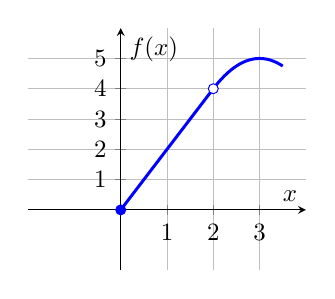
\begin{tikzpicture}[scale=0.9]
\begin{axis}[
  axis lines=middle,
  xmin=-2, xmax=4,
  ymin=-2, ymax=6,
  xtick={0,1,2,3},
  ytick={0,1,2,3,4,5},
  width=5.5cm, height=5cm,
  grid=major,
  xlabel={$x$}, ylabel={$f(x)$}
]
\addplot[very thick, blue, domain=0:2] {2*x};
\addplot[very thick, blue, domain=2:3.5] {-(x-3)^2 + 5};
\addplot[only marks, mark=*, mark options={fill=white}, blue] coordinates {(2,4)};
\addplot[only marks, mark=*, blue] coordinates {(0,0)};
\end{axis}
\end{tikzpicture}
\quad
\begin{tabular}{|c|c|}
\hline
$x$ & $g(x)$ \\\hline
$0$ & $1$ \\
$1$ & $3$ \\
$2$ & $4$ \\
$3$ & $2$ \\\hline
\end{tabular}
\end{center}

What is the value of $(f \cdot g)(1)$?
\begin{hint}
$(f\cdot g)(1) = f(1)\cdot g(1)$. Read $f(1)$ from the graph and $g(1)$ from the table.
\end{hint}
\begin{multipleChoice}
  \choice{$3$}
  \choice[correct]{$6$}
  \choice{$9$}
  \choice{$12$}
\end{multipleChoice}
\end{problem}

\begin{problem}
Let $f(x) = \sqrt{x}$ and $g(x) = x - 5$. What is the domain of $(f \circ g)(x)$?
\begin{hint}
$(f\circ g)(x) = f(g(x)) = \sqrt{x-5}$. The radicand must be non-negative.
\end{hint}
\begin{multipleChoice}
  \choice{$x \geq 0$}
  \choice[correct]{$x \geq 5$}
  \choice{$x > 5$}
  \choice{$x > 0$}
\end{multipleChoice}
\end{problem}

\begin{problem}
Suppose $h(x) = \sqrt{3x+1}$. Which pair of functions satisfies $h(x) = (f\circ g)(x)$?
\begin{hint}
$(f\circ g)(x) = f(g(x))$. The inner function $g$ should produce the argument of the outer function $f$.
\end{hint}
\begin{multipleChoice}
  \choice[correct]{$f(x) = \sqrt{x}$, $g(x) = 3x+1$}
  \choice{$f(x) = 3x+1$, $g(x) = \sqrt{x}$}
  \choice{$f(x) = \sqrt{3x}$, $g(x) = x+1$}
  \choice{$f(x) = \sqrt{x+1}$, $g(x) = 3x$}
\end{multipleChoice}
\end{problem}

\begin{problem}
Let $f(x) = \dfrac{1}{x}$ and $g(x) = x^2 - 4$. Which of the following best describes the domain of $f(g(x))$?
\begin{hint}
$f(g(x)) = \dfrac{1}{x^2-4}$. The denominator cannot be zero; solve $x^2-4=0$.
\end{hint}
\begin{multipleChoice}
  \choice{$(-\infty,\infty)$}
  \choice{$(-2,2)$}
  \choice{$(-\infty,-2)\cup(2,\infty)$}
  \choice[correct]{$(-\infty,-2)\cup(-2,2)\cup(2,\infty)$}
\end{multipleChoice}
\end{problem}

\begin{problem}
Values of $f$ and $g$ are given in the table.
\begin{center}
\begin{tabular}{c|ccccc}
$x$ & $-2$ & $-1$ & $0$ & $1$ & $2$ \\\hline
$f(x)$ & $3$ & $0$ & $-1$ & $4$ & $-2$ \\
$g(x)$ & $1$ & $-2$ & $4$ & $-1$ & $0$
\end{tabular}
\end{center}
Which correctly gives the value of $(f\circ g)(-1)$?
\begin{hint}
$(f\circ g)(-1) = f(g(-1))$. First find $g(-1)$, then evaluate $f$ at that value.
\end{hint}
\begin{multipleChoice}
  \choice[correct]{$f(g(-1)) = f(-2) = 3$}
  \choice{$f(g(-1)) = f(-2) = -2$}
  \choice{$f(g(-1)) = f(2) = -2$}
  \choice{$f(g(-1)) = f(0) = -1$}
\end{multipleChoice}
\end{problem}


\bigskip
\section*{Extended Practice}

\begin{problem}
Given $r(x) = -3x$, $p(x) = x^2+3x$, and $q(z) = \sqrt{1-z}$, evaluate the following. Write \textit{Undefined} where appropriate.
\begin{enumerate}
  \item[(a)] $(p\cdot q)(-1)$
  \medskip
  \item[(b)] $(p+r)(4)$
  \medskip
  \item[(c)] $(p-r)(2)$
  \medskip
  \item[(d)] $\left(\dfrac{r}{q}\right)(1)$
\end{enumerate}

\begin{solution}
\begin{enumerate}
  \item[(a)] $(p\cdot q)(-1) = p(-1)\cdot q(-1) = [(-1)^2+3(-1)]\cdot\sqrt{1-(-1)} = (-2)\sqrt{2} = -2\sqrt{2}$

  \item[(b)] $(p+r)(4) = p(4)+r(4) = [16+12]+[-12] = 28-12 = 16$

  \item[(c)] $(p-r)(2) = p(2)-r(2) = [4+6]-[-6] = 10+6 = 16$

  \item[(d)] $\left(\dfrac{r}{q}\right)(1) = \dfrac{r(1)}{q(1)} = \dfrac{-3}{\sqrt{1-1}} = \dfrac{-3}{0}$ --- \textbf{Undefined.}
\end{enumerate}
\end{solution}
\end{problem}


\begin{problem}
Use the table of values to evaluate the following. Write \textit{Undefined} where appropriate.

\begin{center}
\begin{tabular}{|c|c|c|c|c|c|c|}
\hline
$x$ & $-1$ & 0 & 1 & 2 & 3 & 4 \\\hline
$f(x)$ & $-2$ & 5 & 0 & $-1$ & 2 & $-3$ \\\hline
$g(x)$ & 6 & $-7$ & 3 & 0 & 1 & 2 \\\hline
\end{tabular}
\end{center}

\begin{enumerate}
  \item[(a)] $\left(\dfrac{f}{g}\right)(2)$
  \medskip
  \item[(b)] $(f\cdot g)(4)$
  \medskip
  \item[(c)] $(g\circ f)(2)$
  \medskip
  \item[(d)] $(g-f)(-1)$
\end{enumerate}

\begin{solution}
\begin{enumerate}
  \item[(a)] $\left(\dfrac{f}{g}\right)(2) = \dfrac{f(2)}{g(2)} = \dfrac{-1}{0}$ --- \textbf{Undefined.}

  \item[(b)] $(f\cdot g)(4) = f(4)\cdot g(4) = (-3)(2) = -6$

  \item[(c)] $(g\circ f)(2) = g(f(2)) = g(-1) = 6$

  \item[(d)] $(g-f)(-1) = g(-1)-f(-1) = 6-(-2) = 8$
\end{enumerate}
\end{solution}
\end{problem}


\begin{problem}
Given $s(x) = \dfrac{x-2}{x^2-9}$, $t(x) = \dfrac{x-3}{2-x}$, $v(x) = \sqrt{x+3}$, find each function and its domain.
\begin{enumerate}
  \item[(a)] $(s\cdot t)(x)$
  \medskip
  \item[(b)] $(s\cdot v)(x)$
  \medskip
  \item[(c)] $\left(\dfrac{v}{s}\right)(x)$
\end{enumerate}

\begin{solution}
\begin{enumerate}
  \item[(a)]
  \begin{align*}
    (s\cdot t)(x) &= \frac{x-2}{(x-3)(x+3)}\cdot\frac{x-3}{2-x} = \frac{(x-2)(x-3)}{(x-3)(x+3)(2-x)} = \frac{-1}{x+3}
  \end{align*}
  Domain of $s$: $x\neq\pm3$. Domain of $t$: $x\neq 2$. Intersection: $(-\infty,-3)\cup(-3,2)\cup(2,3)\cup(3,\infty)$.

  \item[(b)]
  $$(s\cdot v)(x) = \frac{(x-2)\sqrt{x+3}}{(x+3)(x-3)}$$
  Domain of $s$: $x\neq\pm3$. Domain of $v$: $x\geq-3$. Intersection: $(-3,3)\cup(3,\infty)$.

  \item[(c)]
  $$\left(\frac{v}{s}\right)(x) = \frac{\sqrt{x+3}}{\dfrac{x-2}{x^2-9}} = \frac{(x^2-9)\sqrt{x+3}}{x-2}$$
  Domain of $v$: $x\geq-3$. Domain of $s$: $x\neq\pm3$. Additionally $s(x)\neq0$ requires $x\neq2$. Intersection: $(-3,2)\cup(2,3)\cup(3,\infty)$.
\end{enumerate}
\end{solution}
\end{problem}


\begin{problem}
Find $(f\circ g)(x)$ and its domain.
\begin{enumerate}
  \item[(a)] $f(x) = \dfrac{4}{x^2-9}$; \quad $g(x) = \sqrt{3-x}$
  \medskip
  \item[(b)] $f(x) = \dfrac{x}{x+4}$; \quad $g(x) = \dfrac{3}{x^2-1}$
\end{enumerate}

\begin{solution}
\begin{enumerate}
  \item[(a)]
  \begin{align*}
    (f\circ g)(x) &= f\!\left(\sqrt{3-x}\right) = \frac{4}{(\sqrt{3-x})^2-9} = \frac{4}{3-x-9} = \frac{4}{-x-6}
  \end{align*}
  Domain of $g$: $x\leq 3$. The simplified composition requires $-x-6\neq0 \Rightarrow x\neq-6$. Domain: $(-\infty,-6)\cup(-6,3]$.

  \item[(b)]
  \begin{align*}
    (f\circ g)(x) &= f\!\left(\frac{3}{x^2-1}\right) = \frac{\dfrac{3}{x^2-1}}{\dfrac{3}{x^2-1}+4} = \frac{3}{3+4(x^2-1)} = \frac{3}{4x^2-1}
  \end{align*}
  Domain of $g$: $x\neq\pm1$. The simplified composition requires $4x^2-1\neq0 \Rightarrow x\neq\pm\dfrac{1}{2}$. Domain: $(-\infty,-1)\cup\!\left(-1,-\tfrac{1}{2}\right)\cup\!\left(-\tfrac{1}{2},\tfrac{1}{2}\right)\cup\!\left(\tfrac{1}{2},1\right)\cup(1,\infty)$.
\end{enumerate}
\end{solution}
\end{problem}


\begin{problem}
Given $q(x) = \dfrac{1}{x-10}$ and $p(x) = x^2-9x$, find $(q\circ q)(x)$ and $(q\circ p)(x)$ and their domains.

\begin{solution}
\begin{itemize}
  \item $(q\circ q)(x) = q\!\left(\dfrac{1}{x-10}\right) = \dfrac{1}{\dfrac{1}{x-10}-10} = \dfrac{x-10}{1-10(x-10)} = \dfrac{x-10}{101-10x}$

  Domain of $q$: $x\neq10$. Simplified form requires $101-10x\neq0 \Rightarrow x\neq10.1$. Domain: $(-\infty,10)\cup(10,10.1)\cup(10.1,\infty)$.

  \item $(q\circ p)(x) = q(x^2-9x) = \dfrac{1}{(x^2-9x)-10} = \dfrac{1}{(x-10)(x+1)}$

  Domain of $p$: all reals. Simplified form requires $x\neq10$ and $x\neq-1$. Domain: $(-\infty,-1)\cup(-1,10)\cup(10,\infty)$.
\end{itemize}
\end{solution}
\end{problem}


\begin{problem}
Find $f(x)$ and $g(x)$ such that $(f\circ g)(x) = h(x)$ and neither $f$ nor $g$ equals $x$.
\begin{enumerate}
  \item[(a)] $h(x) = \sqrt[3]{2x+1}$
  \medskip
  \item[(b)] $h(x) = \dfrac{11}{x-3}$
\end{enumerate}

\begin{solution}
\begin{enumerate}
  \item[(a)] $g(x) = 2x+1$, $f(x) = \sqrt[3]{x}$. Then $f(g(x)) = \sqrt[3]{2x+1}$ ✓

  \item[(b)] $g(x) = x-3$, $f(x) = \dfrac{11}{x}$. Then $f(g(x)) = \dfrac{11}{x-3}$ ✓
\end{enumerate}
\end{solution}
\end{problem}


\begin{problem}
Find the difference quotient $\dfrac{f(x+h)-f(x)}{h}$ and simplify.
\begin{enumerate}
  \item[(a)] $f(x) = \sqrt{x+3}$
  \medskip
  \item[(b)] $f(x) = \dfrac{3}{x}$
\end{enumerate}

\begin{solution}
\begin{enumerate}
  \item[(a)]
  \begin{align*}
    \frac{f(x+h)-f(x)}{h} &= \frac{\sqrt{x+h+3}-\sqrt{x+3}}{h}\cdot\frac{\sqrt{x+h+3}+\sqrt{x+3}}{\sqrt{x+h+3}+\sqrt{x+3}}\\
    &= \frac{(x+h+3)-(x+3)}{h(\sqrt{x+h+3}+\sqrt{x+3})} = \frac{1}{\sqrt{x+h+3}+\sqrt{x+3}}
  \end{align*}

  \item[(b)]
  \begin{align*}
    \frac{f(x+h)-f(x)}{h} &= \frac{\dfrac{3}{x+h}-\dfrac{3}{x}}{h} = \frac{3x-3(x+h)}{hx(x+h)} = \frac{-3h}{hx(x+h)} = \frac{-3}{x(x+h)}
  \end{align*}
\end{enumerate}
\end{solution}
\end{problem}

\end{document}
